\documentclass[]{beamer}
%\documentclass[handout]{beamer}
% ***************************************************************
% for handout, change only this...
%   \documentclass[twocolumn]{article}
%   \usepackage{beamerarticle}
%   \setlength{\textwidth}{7.5in}
%   \setlength{\textheight}{9.8in}
%   \setlength{\topmargin}{-1in}  
%   \setlength{\oddsidemargin}{-.52in}  
%   \setlength{\evensidemargin}{-.52in}  

%\usepackage{beamerprosper}
%\usetheme{Warsaw}
%\usecolortheme{orchid}

\usepackage{graphicx}
\usepackage{amsmath,amssymb,array,comment,eucal}
\newcommand{\e}{\mathbf{e}}
\renewcommand{\P}{\mathbf{P}}
\newcommand{\F}{\mathbf{F}}
\newcommand{\R}{\textsf{R}}
\newcommand{\mat}[1] {\mathbf{#1}}
%\newcommand{\ind}{\mathrel{\mathop{\sim}\limits^{\mathit{ind}}}}
%\newcommand{\iid}{\mathrel{\mathop{\sim}\limits^{\mathit{iid}}}}
\newcommand{\E}{\textsf{E}}
\newcommand{\SE}{\textsf{SE}}
\newcommand{\SSE}{\textsf{SSE}}
\newcommand{\RSS}{\textsf{RSS}}
\newcommand{\FSS}{\textsf{FSS}}
\renewcommand{\SS}{\textsf{SS}}
\newcommand{\MSE}{\textsf{MSE}}
\newcommand{\SSR}{\textsf{SSR}}
\newcommand{\Be}{\textsf{Beta}}
\newcommand{\St}{\textsf{St}}
%\newcommand{\C}{\textsf{C}}
\newcommand{\GDP}{\textsf{GDP}}
\newcommand{\NcSt}{\textsf{NcSt}}
\newcommand{\Bin}{\textsf{Bin}}
\newcommand{\NB}{\textsf{NegBin}}
\renewcommand{\NG}{\textsf{NG}}
\newcommand{\N}{\textsf{N}}
\newcommand{\Ber}{\textsf{Ber}}
\newcommand{\Poi}{\text{Poi}}
\newcommand{\Gam}{\textsf{Gamma}}
\newcommand{\BB}{\textsf{BB}}
\newcommand{\Gm}{\textsf{G}}
\newcommand{\Un}{\textsf{Unif}}
\newcommand{\Ex}{\textsf{Exp}}
\newcommand{\DE}{\textsf{DE}}
\newcommand{\tr}{\textsf{tr}}
\newcommand{\cF}{{\cal{F}}}
\newcommand{\cL}{{\cal{L}}}
\newcommand{\cI}{{\cal{I}}}
\newcommand{\cB}{{\cal{B}}}
\newcommand{\cP}{{\cal{P}}}
\newcommand{\bbR}{\mathbb{R}}
\newcommand{\bbN}{\mathbb{N}}
\newcommand{\pperp}{\mathrel{{\rlap{$\,\perp$}\perp\,\,}}}
\newcommand{\OFP}{(\Omega,\cF, \P)}
\newcommand{\eps}{\boldsymbol{\epsilon}}
\newcommand{\1}{\mathbf{1}_n}
\newcommand{\gap}{\vspace{8mm}}
\newcommand{\ind}{\mathrel{\mathop{\sim}\limits^{\rm ind}}}
\newcommand{\simiid}{\ensuremath{\mathrel{\mathop{\sim}\limits^{\rm
iid}}}}
\newcommand{\eqindis}{\ensuremath{\mathrel{\mathop{=}\limits^{\rm D}}}}
\newcommand{\iid}{\textit{i.i.d.}}
\newcommand{\SSZ}{S_{zz}}
\newcommand{\SZW}{S_{zw}}
\newcommand{\Var}{\textsf{Var}}
\newcommand{\corr}{\textsf{corr}}
\newcommand{\diag}{\textsf{diag}}
\newcommand{\var}{\textsf{var}}
\newcommand{\Cov}{\textsf{Cov}}
\newcommand{\Sam}{{\cal S}}
\def\H{\mathbf{H}}
\newcommand{\I}{\mathbf{I}}
\newcommand{\Y}{\mathbf{Y}}
\newcommand{\tY}{\tilde{\mathbf{Y}}}
\newcommand{\Yhat}{\hat{\mathbf{Y}}}
\newcommand{\Yobs}{\mathbf{Y}_{{\cal S}}}
\newcommand{\barYobs}{\bar{Y}_{{\cal S}}}
\newcommand{\barYmiss}{\bar{Y}_{{\cal S}^c}}
\def\bv{\mathbf{b}}
\def\X{\mathbf{X}}
\def\tX{\tilde{\mathbf{X}}}
\def\x{\mathbf{x}}
\def\xbar{\bar{\mathbf{x}}}
\def\Xbar{\bar{\mathbf{X}}}
\def\Xg{\mathbf{X}_{\boldsymbol{\gamma}}}
\def\Ybar{\bar{\Y}}
\def\ybar{\bar{y}}
\def\y{\mathbf{y}}
\def\Yf{\mathbf{Y_f}}
\def\W{\mathbf{W}}
\def\L{\mathbf{L}}
\def\w{\mathbf{w}}
\def\U{\mathbf{U}}
\def\V{\mathbf{V}}
\def\Q{\mathbf{Q}}
\def\Z{\mathbf{Z}}
\def\z{\mathbf{z}}
\def\v{\mathbf{v}}
\def\u{\mathbf{u}}

\def\zero{\mathbf{0}}
\def\one{\mathbf{1}}
\newcommand{\taub}{\boldsymbol{\tau}}
\newcommand{\betav}{\boldsymbol{\beta}}
\newcommand{\alphav}{\boldsymbol{\alpha}}
\newcommand{\A}{\mathbf{A}}
\def\a{\mathbf{a}}
\def\K{\mathbf{K}}
\newcommand{\B}{\mathbf{B}}
\def\b{\boldsymbol{\beta}}
\def\bhat{\hat{\boldsymbol{\beta}}}
\def\btilde{\tilde{\boldsymbol{\beta}}}
\def\tb{\tilde{\boldsymbol{\beta}}}
\def\bg{\boldsymbol{\beta_\gamma}}
\def\bgnot{\boldsymbol{\beta_{(-\gamma)}}}
\def\mub{\boldsymbol{\mu}}
\def\tmub{\tilde{\boldsymbol{\mu}}}
\def\muhat{\hat{\boldsymbol{\mu}}}
\def\t{\boldsymbol{\theta}}
\def\tk{\boldsymbol{\theta}_k}
\def\tj{\boldsymbol{\theta}_j}
\def\Mk{\boldsymbol{{\cal M}}_k}
\def\M{\boldsymbol{{\cal M}}}
\def\Mj{\boldsymbol{{\cal M}}_j}
\def\Mi{\boldsymbol{{\cal M}}_i}
\def\Mg{{\boldsymbol{{\cal M}_\gamma}}}
\def\Mnull{\boldsymbol{{\cal M}}_{N}}
\def\gMPM{\boldsymbol{\gamma}_{\text{MPM}}}
\def\gHPM{\boldsymbol{\gamma}_{\text{HPM}}}
\def\Mfull{\boldsymbol{{\cal M}}_{F}}
\def\tg{\boldsymbol{\theta}_{\boldsymbol{\gamma}}}
\def\g{\boldsymbol{\gamma}}
\def\eg{\boldsymbol{\eta}_{\boldsymbol{\gamma}}}
\def\G{\mathbf{G}}
\def\cM{\cal M}
\def\D{\Delta}
\def \shat{{\hat{\sigma}}^2}
\def\uv{\mathbf{u}}
\def\l {\lambda}
\def\d{\delta}
\def\Sigmab{\boldsymbol{\Sigma}}
\def\Lambdab{\boldsymbol{\Lambda}}
\def\lambdab{\boldsymbol{\lambda}}
\def\Mg{{\cal M}_\gamma}
\def\S{{\cal{S}}}
\def\qg{p_{\boldsymbol{\gamma}}}
\def\pg{p_{\boldsymbol{\gamma}}}
\def\t{\boldsymbol{\theta}}  
\def\T{\boldsymbol{\Theta}}  
\title{BMA}

\author{Hoff Chapter 9, Liang et al 2007, Hoeting et al (1999), Clyde \&
 George (2004)} 
\date{\today}
%\Logo(-1.9,7.3){\includegraphics[width=.5in]{../eps/duke}}
% Optional: text to put in the bottom of each slide.
% By default, the title of the talk will be placed there.
%\slideCaption{\textit{October 28, 2005 }}

\begin{document}
% make the title slide
\maketitle

\begin{frame}\frametitle{Prior Distributions}
  \begin{itemize}

  \item Bayesian Model choice requires  proper prior distributions on
  regression coefficients that are not common to all models\pause 
\vspace{2in}

\item Vague but proper priors  may lead to paradoxes!  (Lindley \& Bartlett) \pause 

  \end{itemize}
\end{frame}

\begin{frame}\frametitle{Prior Distributions}
  \begin{itemize}
  \item ``Spike and Slab'' - Lempers (1971) Mitchell \& Beauchamp (1988) \pause 
  \item ``Spike and Bell''  Leamer (1978)  in BMA \pause
  \item   mixture of 2 normals - concentrated and dispersed - SSVS Gibbs Sampler -  George \& McCulloch (1993) \pause
\item Back to ``Spike and Bell''  Hoeting, Raftery \& Madigan $MC^3$ (1997) and George  (1997) collapsed MCMC integrate out $\bg$
  \item Conjugate Normal-Gammas lead to closed form expressions for
  marginal likelihoods, Zellner's g-prior is the most popular. \pause 
  \end{itemize}
\end{frame}

\begin{frame}\frametitle{Zellner's g-prior}
  Centered model:  $$\Y = \1 \alpha + \X^c \b + \epsilon$$  
  where $\X^c$ is the centered design matrix where all variables have
  had their mean subtracted \pause 
\begin{itemize}
\item   $p(\alpha) \propto 1$ \pause 
\item  $p(\sigma^2) \propto 1/\sigma^2$  \pause 
\item  $\b_\gamma \mid \alpha, \sigma^2, \g \sim \N(0, g \sigma^2
  ({\Xg^c}^\prime \Xg^c)^{-1})$ \pause 
%\item  take $g=n$
\end{itemize}
which leads to marginal likelihood of $\Mg$ that is proportional
to $$ p(\Y \mid \Mg) = C (1 + g)^{\frac{n-p-1}{2}} ( 1 + g (1 -
 R^2_\gamma))^{- \frac{(n-1)}{2}}$$
where $R^2$ is the usual $R^2$ for model $\Mg$.
\pause 

Trade-off of model complexity versus goodness of fit

\bigskip
Lastly, assign distribution to space of models
\end{frame}

\begin{frame}
  \frametitle{Priors on Model Space}
  $p(\Mg) \Leftrightarrow p(\g)$
  \begin{itemize}
  \item $p(\gamma_j = 1) = .5 \Rightarrow P(\Mg) = .5^p$  Uniform on space of models \pause $\pg \sim \Bin(p, .5)$
\item $\gamma_j \mid \pi \simiid \Ber(\pi)$ and $\pi \sim \Be(a,b)$ then  $\pg \sim \BB(p, a, b)$
$$
p(\pg \mid p, a, b) = \frac{ \Gamma(p + 1) \Gamma(\pg + a) \Gamma(p - \pg + b) \Gamma (a + b) }{\Gamma(\pg+1) \Gamma(p - \pg + 1) \Gamma(p + a + b) \Gamma(a) \Gamma(b)}
$$
\item $\pg \sim \BB(p, 1, 1) \sim \Un(0, p)$
\item For sparsity. want $b$ to be a function of $p$ typically. 
  \end{itemize}
\end{frame}

\begin{frame}[fragile]
\frametitle{USair Data}
\begin{verbatim}
library(BAS)
poll.bma = bas.lm(log(SO2) ~ temp + log(firms) + 
                             log(popn) + wind + 
                             precip+ rain, 
                  data=pollution, 
                  prior="g-prior", 
                  alpha=41,
                  n.models=2^6, 
                  modelprior = uniform(),
                  update=50, 
                  initprobs="Uniform")
> poll.bma

 Marginal Posterior Inclusion Probabilities: 
 Intercept  temp   log(mfgfirms)  log(popn)   wind  precip  raindays
   1.0000   0.9755       0.7190     0.2757  0.7654  0.5994   0.3104  
\end{verbatim}
\end{frame}
\begin{frame}[fragile]\frametitle{Plots}
plot(poll.bma, ask=F)
  \centering 
  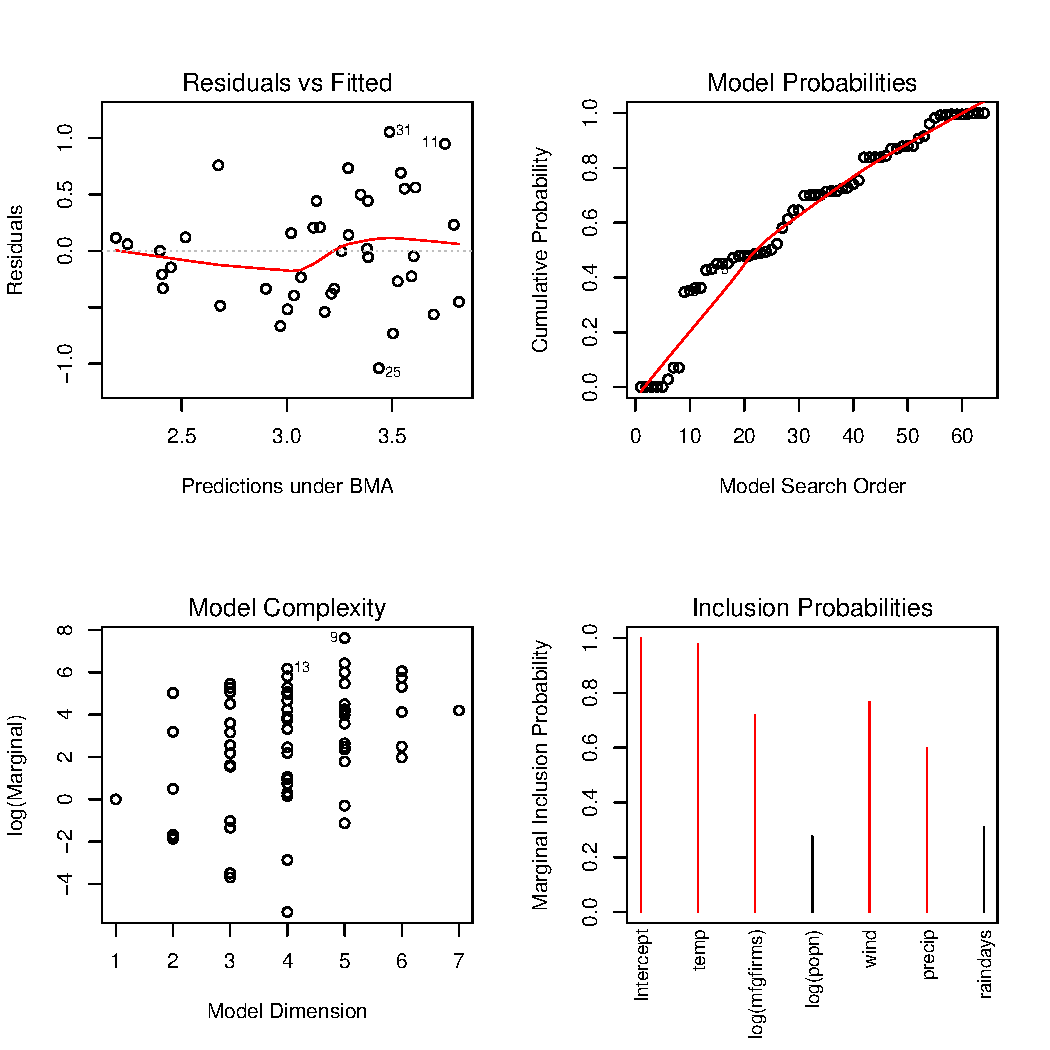
\includegraphics[height=3.5in]{poll-bma-sum}
\end{frame}

\begin{frame}\frametitle{Posterior Distribution  with Uniform Prior on Model Space}
image(poll.bma)

\centering
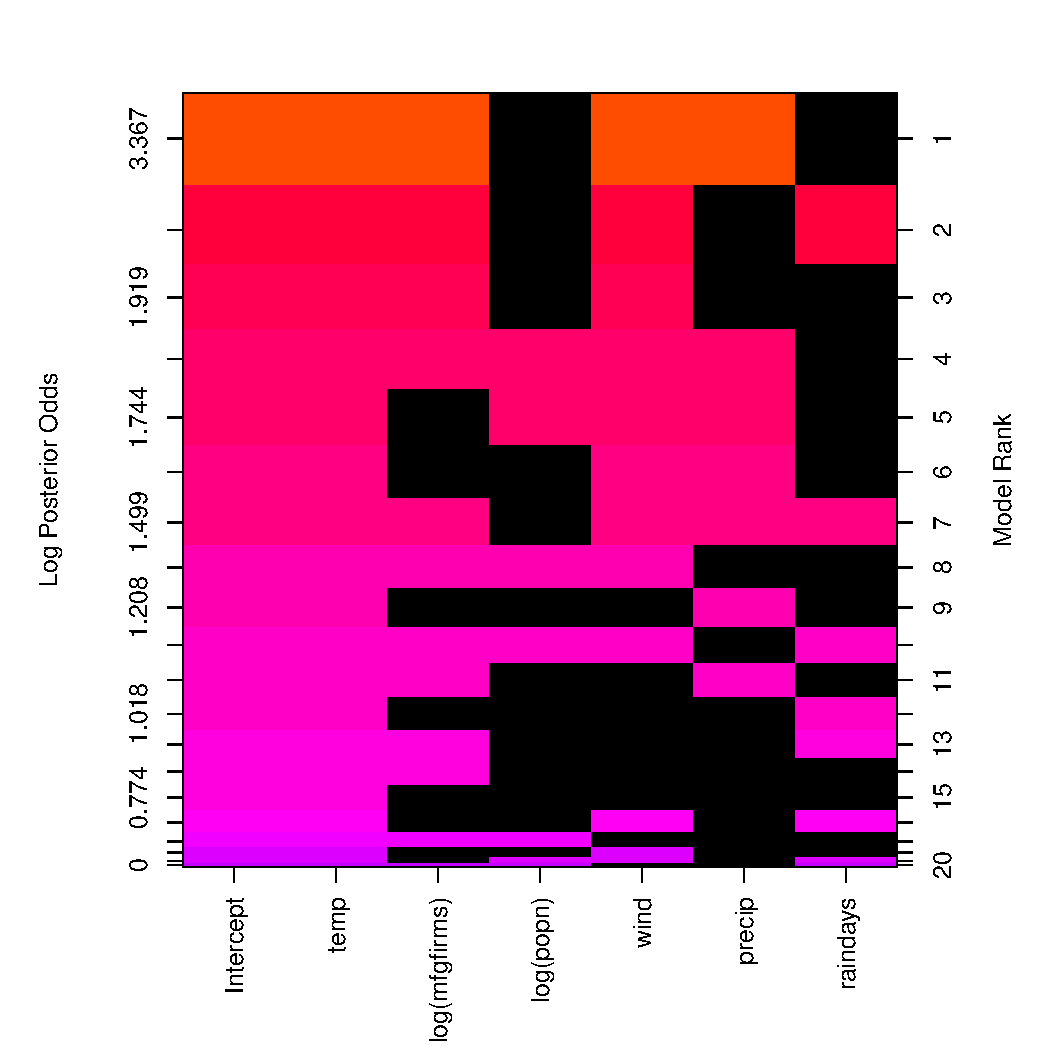
\includegraphics[height=3.5in]{poll-image}  
\end{frame}

\begin{frame}\frametitle{Posterior Distribution  with BB(1,p) Prior on Model Space}
image(poll-bb.bma)

\centering
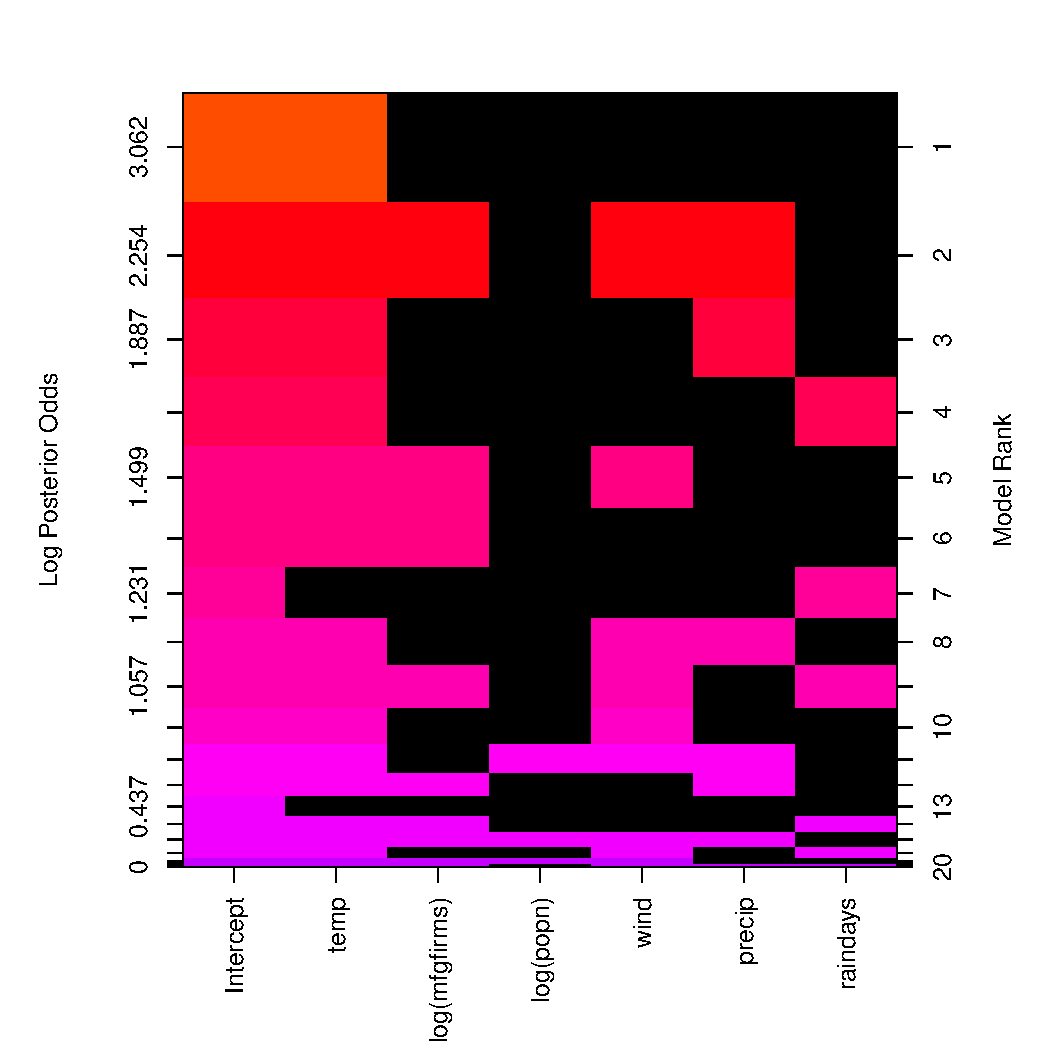
\includegraphics[height=3.5in]{poll-bb-image}  
\end{frame}


\begin{frame}
\frametitle{Jeffreys Scale of Evidence}
\begin{itemize}
\item Bayes Factor = ratio of marginal likelihoods \pause

\item Posterior odds = Bayes Factor $\times$ Prior odds \pause

\end{itemize}


$B = BF[\M_0 : \Mg]$   and $1/B = BF[\Mg : \M_0]$ \pause

\vspace{14pt}

\begin{tabular}{|r|l|} \hline \hline
Bayes Factor & Interpretation \\ \hline
$B \geq 1$ & $H_0$ supported \\
$1 > B \geq 10^{-\frac{1}{2}} $ & minimal evidence against $H_0$ \\
$ 10^{- \frac{1}{2}} > B  \geq 10^{-1}$ & substantial evidence against $H_0$ \\
$ 10^{-1} > B  \geq 10^{-2}$ & strong evidence against $H_0$ \\
$ 10^{-2} > B $ & decisive evidence against $H_0$ \\ \hline \hline
\end{tabular}
\pause
in context of testing one hypothesis with equal prior odds
\end{frame}


\begin{frame}[fragile]
\frametitle{Coefficients}
\begin{verbatim}
 beta = coef(poll.bma)
 par(mfrow=c(2,3));  plot(beta, subset=2:7,ask=F)
\end{verbatim}
\centering
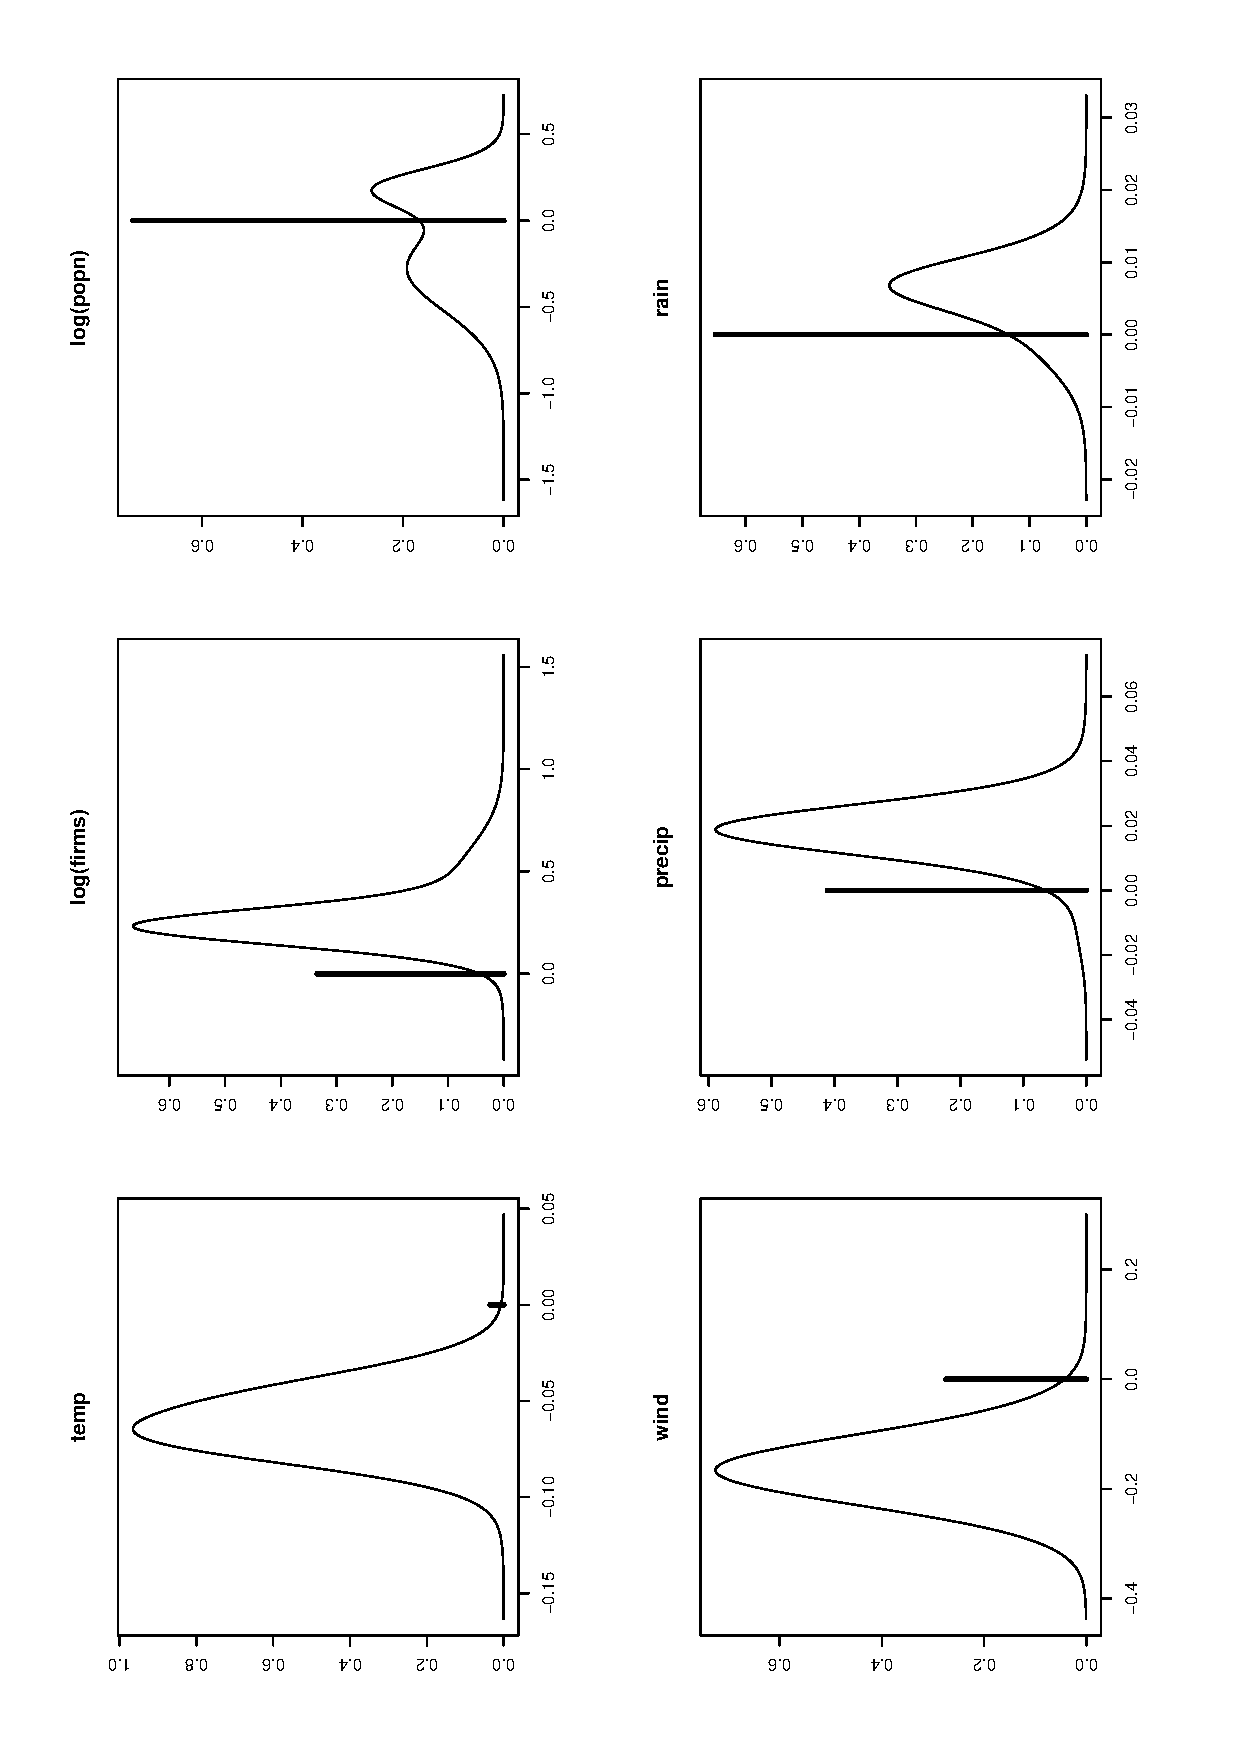
\includegraphics[height=3in]{poll-beta}  

\end{frame}

\begin{frame}
  \frametitle{Information Paradox}
  
The Bayes factor for comparing $\Mg$ to the null
model:
$$
 BF(\Mg : \M_0) =    (1 + g)^{(n - 1 - \pg)/2} (1 + g(1 - R^2))^{-(n-1)/2}
$$
\pause
\begin{itemize}
\item Let $g$ be a fixed constant and take $n$ fixed. \pause
\item Let $F = \frac{R_{\g}^2/\pg}{(1 - R_{\g}^2)/(n - 1 - \pg)}$ \pause
\item As $R^2_{\g} \to 1$, $F \to \infty$ LR test would reject $\M_0$
  where $F$ is the usual $F$ statistic for  comparing model $\Mg$ to
  $\M_0$ \pause 
\item BF converges to a fixed constant $(1+g)^{-\pg/2}$  (does not go
  to infinity
\end{itemize}

``Information Inconsistency''  see Liang et al JASA 2008


\end{frame}
\begin{frame}
  \frametitle{Mixtures of $g$ priors \& Information consistency}
  
Need $BF \to \infty$ if $\R^2 \to 1$  $\Leftrightarrow$ $\E_g[(1 +
g)^{-\pg/2}]$ diverges  (proof in Liang et al)
\pause
\begin{itemize}
\item Zellner-Siow Cauchy prior \pause
\item hyper-g prior (Liang et al JASA 2008) \pause
\item robust prior (Bayarrri et al Annals of Statistics 2012 \pause
\end{itemize}

 All have tails that behave like a Cauchy distribution
\end{frame}
\section{Mortality}
\begin{frame}[fragile]
\frametitle{Mortality \& Pollution}
  \begin{itemize}
  \item Data from Statistical Sleuth 12.17 \pause 
  \item 60 cities \pause 
\item response Mortality \pause 
\item measures of HC, NOX, SO2 \pause 
\item Is pollution associated with mortality after adjusting for other
  socio-economic and meteorological factors? \pause 
\item 15 predictor variables implies $2^{15} = 32,768$ possible models
  \pause 
\item Use Zellner-Siow Cauchy prior  $1/g \sim  G(1/2, n/2)$
  \end{itemize}
\begin{verbatim}
mort.bma = bas.lm(MORTALITY ~ ., data=mortality,
                  prior="ZS-null", 
                  alpha=60,  n.models=2^15, 
                  update=100, initprobs="eplogp")
\end{verbatim}
\end{frame}

\begin{frame}\frametitle{Posterior Distributions}
  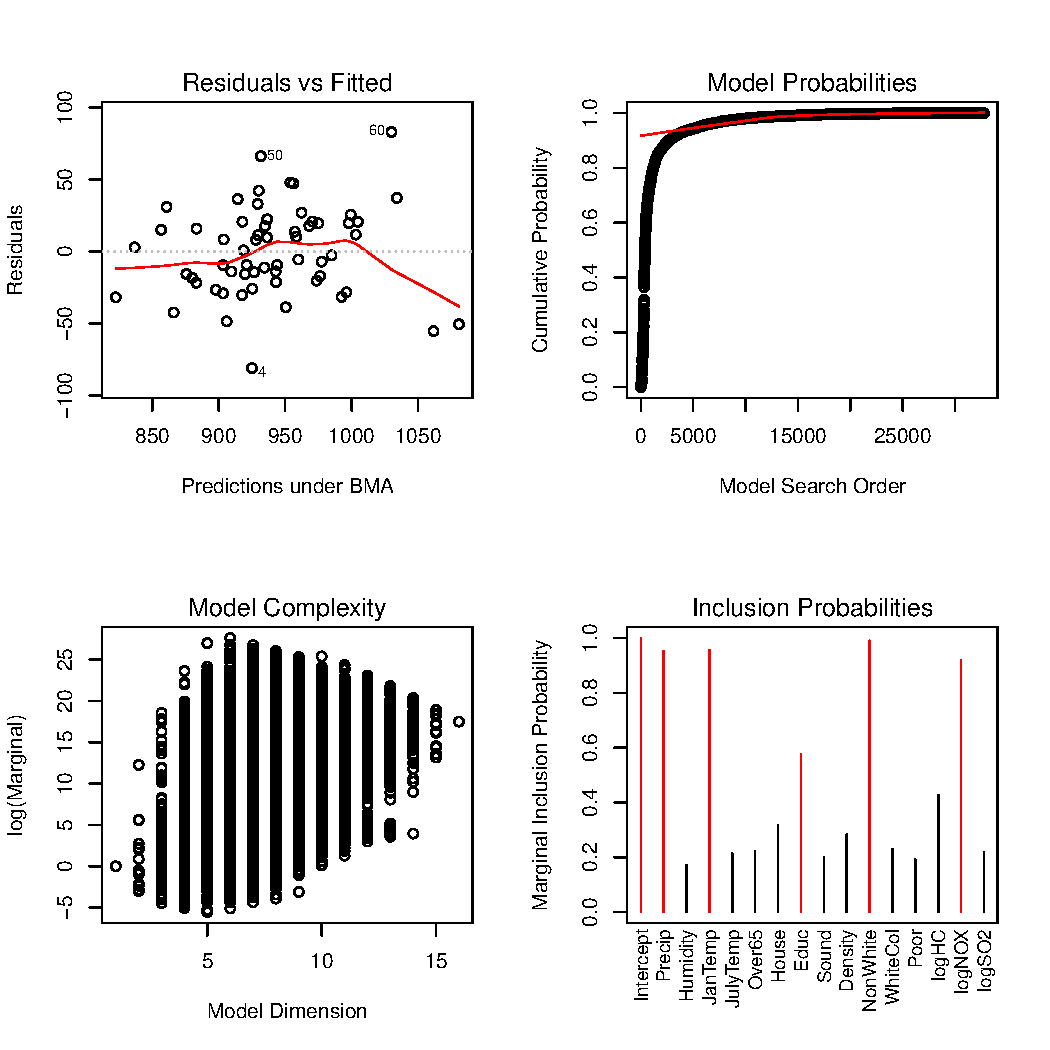
\includegraphics[height=3.5in]{mort-sum}
\end{frame}



\begin{frame}[fragile]
\frametitle{Posterior Probabilities}
  \begin{itemize}
  \item What is the probability that there is no pollution effect? \pause 
\item Sum posterior model probabilities over all models that include
  no pollution variables \pause 
\begin{verbatim}
> which.mat = list2matrix.which(mort.bma,1:(2^15))
> poll.in = (which.mat[, 14:16] %*% rep(1, 3)) > 0
> sum(poll.in * mort.bma$postprob)
[1] 0.9889641
\end{verbatim}\pause 
\item Posterior probability is $0.011$ \pause 
\item Odds that there is an effect  $(1 - .011)/(.011) = 89.$ \pause 
\item Prior Odds $7 = (1 - .5^3)/.5^3$ \pause 
\item Bayes Factor for a pollution effect $ 89.9/7 = 12.8$ \pause 
\item Bayes Factor for NOX based on marginal inclusion probability
  $0.917/(1 - 0.917) = 11.0$ \pause  
\item Marginal inclusion probability for logHC =  0.427144
\item Marginal inclusion probability for logSO2 = 0.218978
\end{itemize}
Bayes Factors are not additive!   Better to work with probabilities...
\end{frame}
\begin{frame}\frametitle{Model Space}
  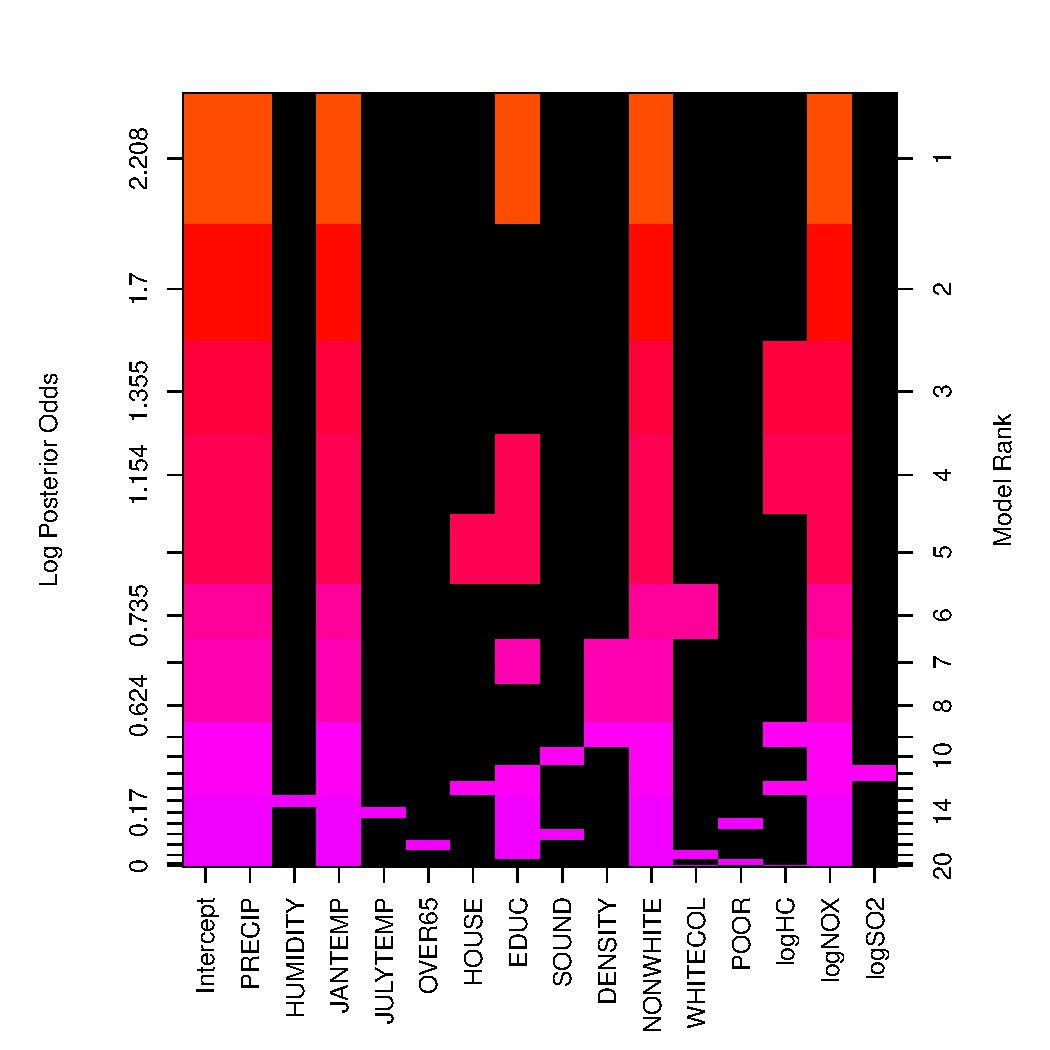
\includegraphics[height=3.5in]{mort-image}
\end{frame}
\begin{frame}\frametitle{Coefficients}
  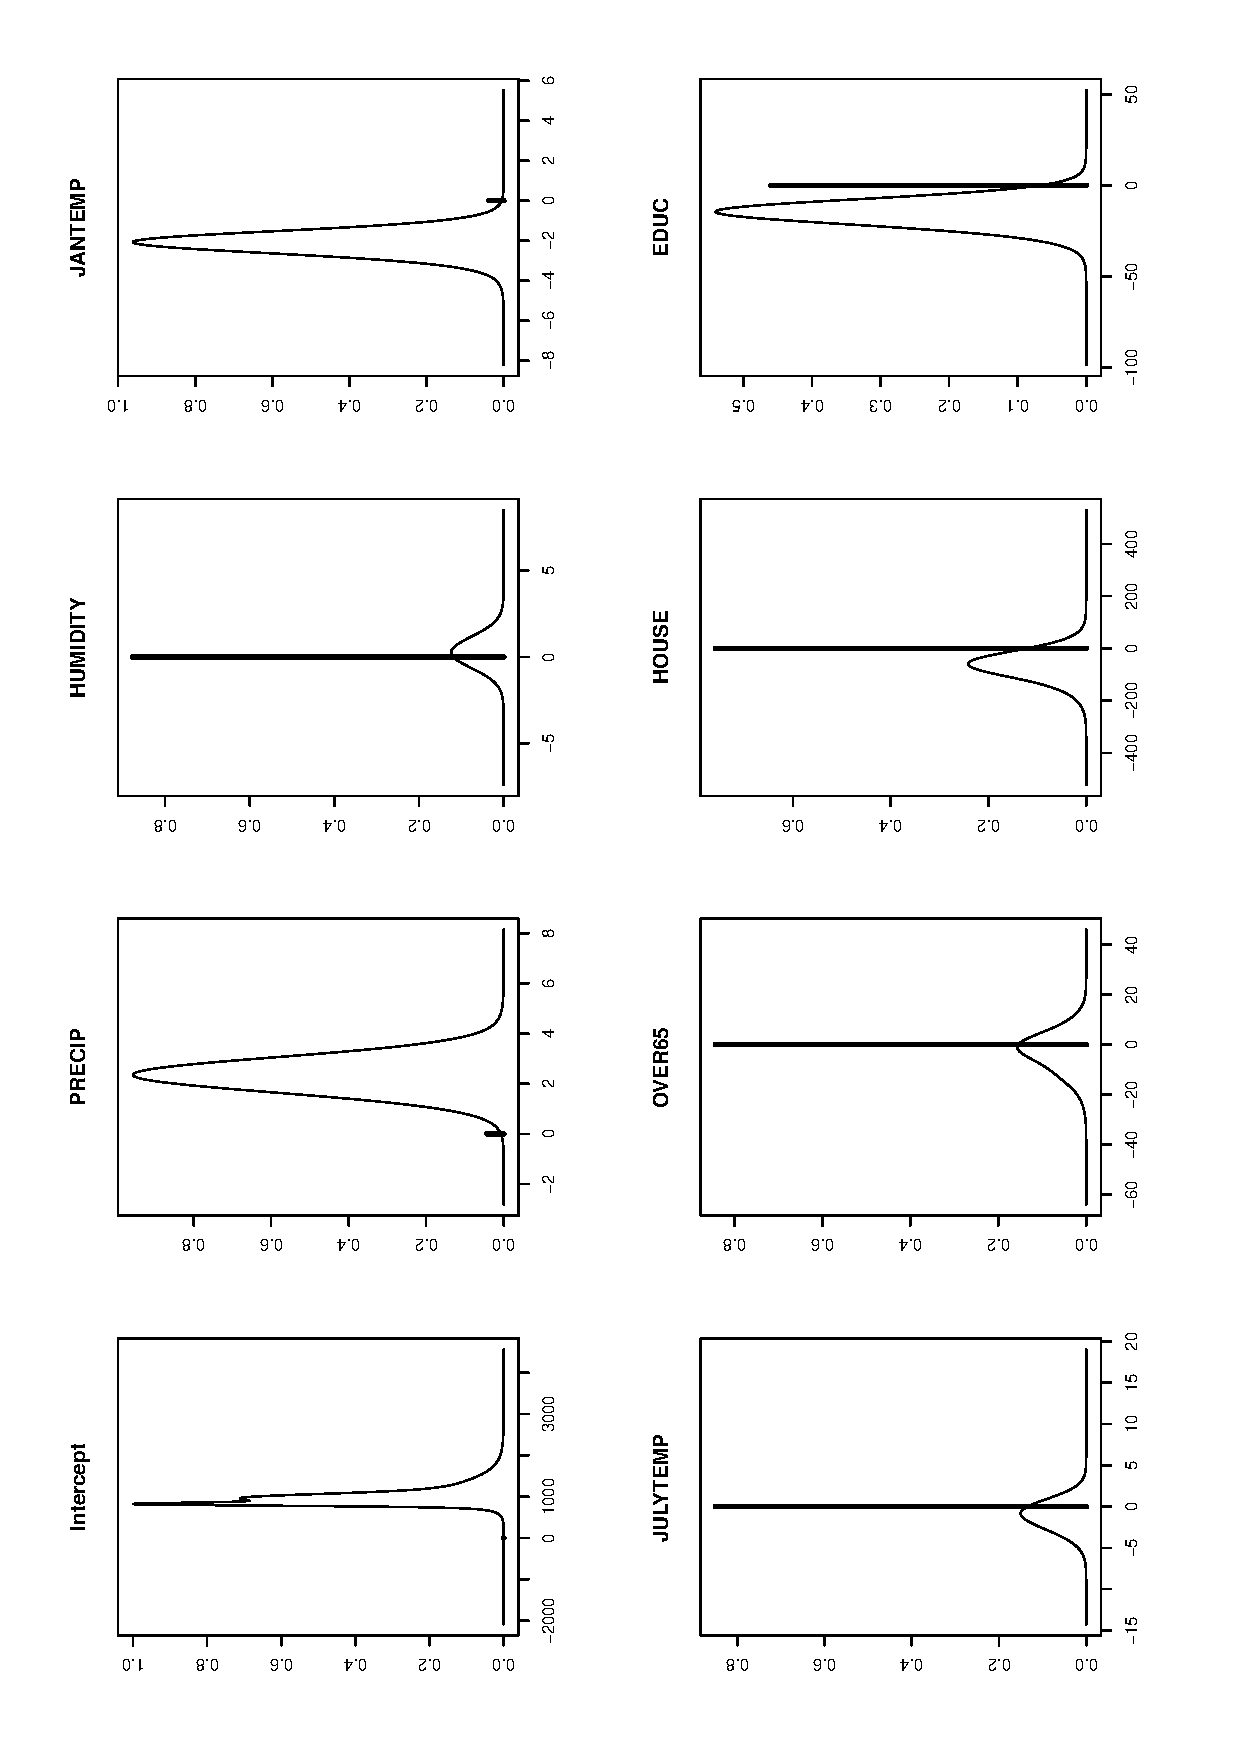
\includegraphics[height=3.5in]{mort-beta1}
\end{frame}

\begin{frame}\frametitle{Coefficients}
  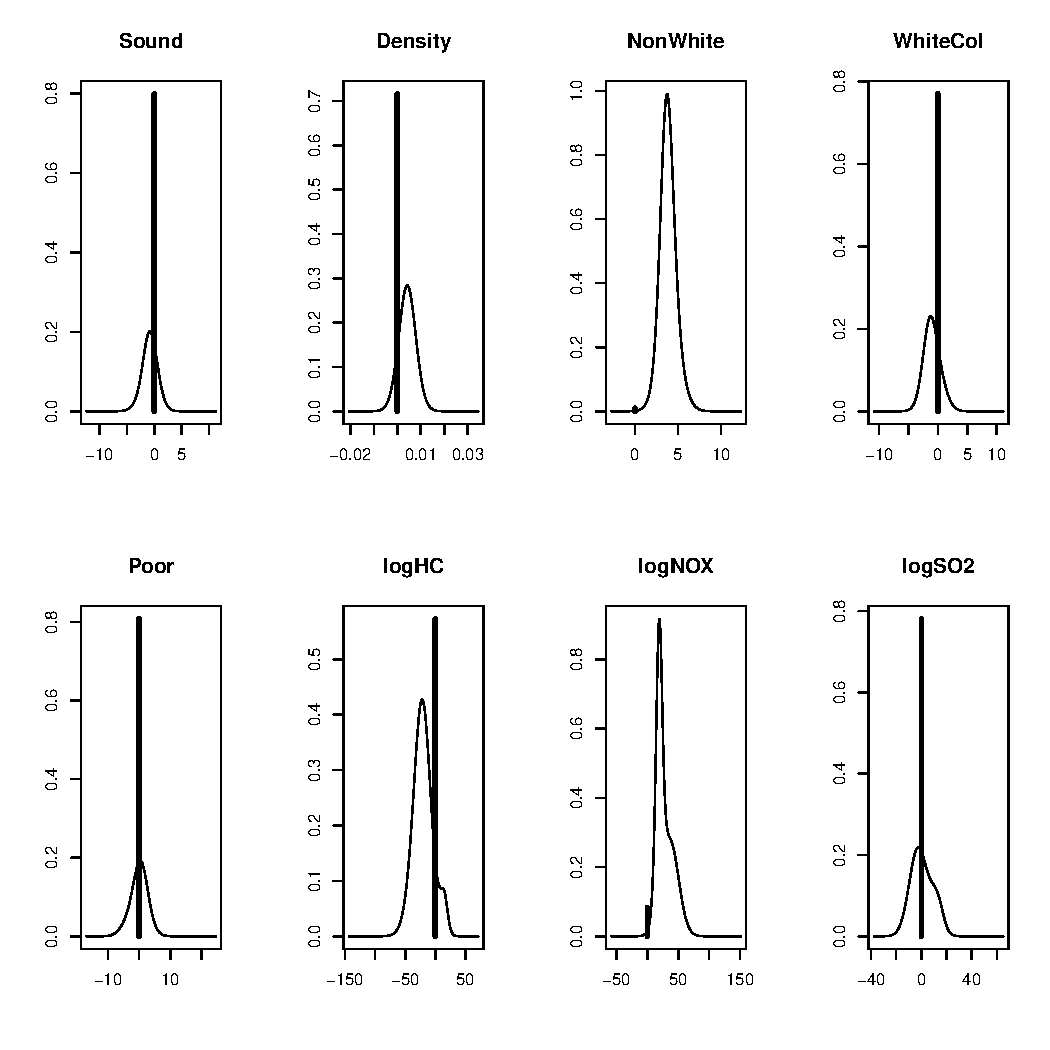
\includegraphics[height=3.5in]{mort-beta2}
\end{frame}

\begin{frame}
  \frametitle{Effect Estimation}
  \begin{itemize}
  \item  Coefficients in each model are adjusted for other variables
    in the model
\item OLS:  leave out a predictor with a non-zero coefficient then
  estimates are biased!
\item Model Selection in the presence of high correlation, may leave
  out "redundant" variables; 
\item improved MSE for prediction (Bias-variance tradeoff)
\item Bayes is biased anyway so should we care?
\item What is meaning of $\sum_{\g} \beta_{j \g} \gamma_j P(\Mg \mid \Y)$
  \end{itemize}
  Problem with confounding!  Need to change prior?

\end{frame}



\begin{frame}\frametitle{ Other Problems}


  \begin{itemize}
  \item Computational \pause 
  if $p > 35$  enumeration is difficult \pause 
  \begin{itemize}
  \item Gibbs sampler or Random-Walk algorithm on $\g$ \pause 
  \item poor convergence/mixing with high correlations \pause 
  \item Metropolis Hastings algorithms more flexibility \pause 
  \item "Stochastic Search" (no guarantee samples represent posterior) \pause 
  \item in BMA all variables are included, but coefficients are 
   shrunk to 0; alternative is to use Shrinkage methods \pause 
  \end{itemize}
\item Prior Choice: Choice of prior distributions on $\b$ and on $\g$ \pause 
\end{itemize}

\bigskip Model averaging versus Model Selection  -- what are objectives?


\end{frame}
\end{document}